% \begin{document}
\chapter{Reti di Flusso}

Innanzi tutto inziamo con alcune definzioni:
\dfn{Rete}{
  definiamo \textbf{rete} un grafo \textit{pesato} $ G = (N,A) $ dove
  \begin{itemize}
    \item $ N $ e' l'insieme dei nodi
    \item $ A $ e' l'insieme degli archi
  \end{itemize}
}

Più precisamente:
\begin{itemize}
  \item $\forall i \in N$ è associato un valore reale $b_i$, detto \textit{sbilanciamento} che può essere:
  \begin{itemize}
    \item \textbf{Positivo}: il nodo $i$ è detto \textit{pozzo} e rappresenta la qunatità del bene che esce della rete al nodo $i$, mentre $b_i$ è ldetto \textit{domanda del bene}
    \item \textbf{Negativo}: il nodo $i$ è detto \textit{sorgente} e rappresenta la quantità del bene che entra nella rete al nodo $i$, mentre $-b_i$ è detto \textit{offerta del bene}
    \item \textbf{Nullo}: il nodo $i$ è detto \textit{transito} e rappresenta un nodo di passaggio
  \end{itemize}
  \item $\forall (i,j) \in A$ è associato un valore reale $c_{ij}$ detto \textit{costo} che rappresenta il costo di trasportare una unità di bene lungo l'arco $(i,j)$ ed una coppia di valori $l_{ij}$ e $u_{ij}$ detti \textit{capacità inferiore} e \textit{capacità superiore} rispettivamente, che rappresentano il minimo e il massimo numero di unità di bene che possono essere trasportate lungo l'arco $(i,j)$
  \begin{center}
    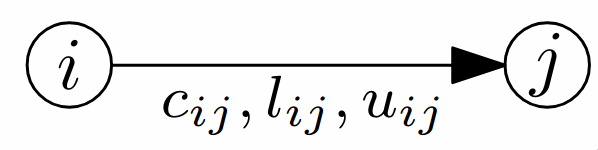
\includegraphics[width=0.5\textwidth]{img/2025-03-05-09-34-49.png}
  \end{center}
\end{itemize}

\section{Problemi di Flusso}
\dfn{Problemi di flusso}{
  > Si definiscono \textit{problemi di flusso} quei problemi che consistono nel determinare, lungo una rete, il flusso di un bene, ossia un assegnamento a ciascun arco \( (i,j) \in A \) un valore reale \( x_{ij} \in [l_{ij}, u_{ij}] \), rispettando i vincoli di capacità e conservazione del flusso
}

\textbf{flusso}, quindi, e' proprio la soluzione che vogliamo trovare. Tuttavia ad ogni unità di flusso assegnata ad un arco corrisponde un costo $c_{ij}$, si ha quindi che il costo complessivo del flusso e' dato da:
\begin{equation}  
  \sum_{(i,j) \in A} c_{ij}x_{ij}
\end{equation}


\subsection{Vincoli}
I vincoli che nei problemi di flusso si deve rispettare sono:
\begin{itemize}
\item \textit{Uguaglianza di domanda e offerta globale}:
  \begin{equation}
    \sum_{i \in D}b_i = - \sum_{i \in O} b_i \iff \sum_{i \in N} b_i = 0
  \end{equation}
  Dove $ D = \{b_i \in N \mid b_i > 0\} $ e $ O = \{b_i \in N \mid b_i < 0\} $. Per quelli nulli, tanto vale non metterli da nessuna parte per non creare asimmetria inutile.
\item \textit{Conservazione di flusso}:
  \begin{quote}
    lol 
    \hfill \textit{Il Basta}
  \end{quote}

  \begin{equation}
    \sum_{(i,j) \in BS(i)} x_{ij} - \sum_{(i,j) \in FS(i)} x_{ij} = b_i \quad \forall i \in N
  \end{equation}
  
dove
\begin{align*}
  BS(i) = \{(k,i) | (k,i) \in A\} \text{ detto stella entrante}\\
  FS(i) = \{(i,k) | (i,k) \in A\} \text{ detto stella uscente}
\end{align*}
Ovvero ciò che entra nel nodo e' uguale a cio' che esce piu' lo sbilanciamento.
\item \textit{Ammissibilità del flusso}:
  \[
    l_{ij} \leq x_{ij} \leq u_{ij} \quad \forall (i,j) \in A
  \]
\end{itemize}



\ex{Esempio di rete}{
  \begin{center}
    \begin{tikzpicture}[
        node distance=2cm,
        vertex/.style={circle, draw, minimum size=1cm},
        edge/.style={->, >=Stealth, auto},
    ]

    % Nodes
    \node[vertex] (1) {1};
    \node[vertex, below=of 1] (2) {2};
    \node[vertex, right=of 1] (3) {3};
    \node[vertex, below=of 3] (4) {4};

    % Edges
    \draw[edge] (1) -- node[above] {3, 1, 4} (3);
    \draw[edge] (1) -- node[left] {4, 0, 6} (2);
    \draw[edge] (2) -- node[below] {1, 2, 5} (4);
    \draw[edge] (3) -- node[right] {3, 1, 10} (4);

    % Labels
    \node[above left=0.1cm of 1] {3};
    \node[below left=0.1cm of 2] {4};
    \node[above right=0.1cm of 3] {2};
    \node[below right=0.1cm of 4] {5};

    \end{tikzpicture}
  \end{center}  
}

Perche' mai dovremmo studiare sta roba? 
\begin{itemize}
\item \textbf{Espressivita'}: permette di catturare un range di problemi concreti abbastanza grande
\item \textbf{Complessita'}: esistono algoritmi che risolvono questo tipo di problemi con complessita' polinomiale abbastanza basso. A Ugo questo fa molto piacere :), perché ricordiamolo NON SIAMO INGENERI GESTIONALI, SIAMO INFORMATICI
\end{itemize}

\subsection{Ipotesi semplificative}

Le ipotesi semplificative sono supposizioni che non consentono di usare il caso generale, ma che semplificano il problema \textbf{senza} perdere espressivita', come ad esempio nel caso in cui le capacita' inferiori sono nulle ovvero $l_{ij}=0$, che e' una situazione a cui possiamo arrivare \textbf{anche da grafi che non hanno questa caratteristica}. 

Infatti data una rete $G$, si può costruire una rete $G'$ tale che $G$ e $G'$ hanno lo stesso flusso ottimo, ma $G'$ ha capacita' inferiori nulle. $\forall (i,j)\in A$:
\begin{itemize}
\item Si sottrae $ l_{ij} $ a $ b_j $ e a $ u_{ij} $
\item Si aggiunge $ l_{ij} $ a $ b_i $
\item Occorre aggiungere la quantita'
  \[
    \sum_{(i,j) \in A} c_{ij}l_{ij}
  \]
  Alla funzione abbiettivo 
\end{itemize}
\nt{
  Si noti che non cambia la soluzione ottima, ma solo il valore ottimo della funzione obbiettivo
}

È pertanto vero, quindi, che ad un flusso $x_{ij} \in H $ corrisponde un flusso $(x_{ij}+l_{ij}) \in G$
\subsection{Problema del Flusso di Costo Minimo}

\dfn{Problema del Flusso di Costo Minimo}{
  Si definisce \textit{problema del flusso di costo minimo} il problema di flusso in cui la funzione obbiettivo è il costo di flusso da minimizzare e le cui capacità inferiori sono nulle
}

Questo problema è formalizzabile in programmazione lineare come segue:
\begin{equation}
  \begin{aligned}
    \min &cx\\ 
    Ex &= b \quad \leq x \leq u  
  \end{aligned}
\end{equation}
dove

\begin{itemize}
  \item $x \in \mathbb{R}^{|A|} $ è il vettore delle variabili di flusso
  \item $c \in \mathbb{R}^{|A|} $ è il vettore dei costi
  \item $E \in \mathbb{R} ^{|N| \times |A|} $ e' una matrice di incidenza fra nodi e archi i cui elementi possono solo assumere valori 0, -1 e 1
  \item $b \in \mathbb{R}^{|N|} $ e' il vettore degli sbilanciamenti
  \item $u \in \mathbb{R}^{|A|}$ e' il vettore delle capacita' superiori
\end{itemize}

In questo modo abbiamo scritto funzione obbiettivo e vincola in forme matriciali molto semplici, adesso, senza terrorizzare nessuno, fornirò la formalizzazione in forma estesa:
\begin{equation}
  \begin{aligned}
    \min &\sum_{(i,j) \in A} c_{ij}x_{ij}\\
    &\sum_{(j,i)\in BS(i)}x_{ji} -\sum_{(i,j) \in A} x_{ij} = b_i \quad \forall i \in N\\
    &l_{ij} \leq x_{ij} \leq u_{ij} \quad \forall (i,j) \in A
  \end{aligned}
\end{equation}

\subsubsection{Rilassamento di assunzioni}
Puo' essere utile assumere che esiste un solo pozzo e una sola sorgente, che vengono poi collegati con archi fittizi (a costo nullo e capacita' pari allo sbilanciamento dei pozzi/sorgenti effettivi!) a quelli effettivi. 

\begin{quote}
  Non si può, però, enunciare che i nodi non hanno una capacita', perche' di fatto non succede nulla, perche' puo' essere trasformata in una rete equivalente dove i nodi non ce l'hanno:

  \hfill \textit{TODO: spiegare meglio, che cazzo vuoi dire ibbastianini?}
\end{quote}

Per trasformare un generico problema MCF in un problema con una sola sorgente ed un solo pozzo_
\begin{itemize}
  \item Si aggiungono due nodi fittizi $s$ e $t$, uno sorgente e uno pozzo
  \item Si aggiungono archi fittizi  da $s$ ai nodi sorgenti di partenza, con un costo nullo e capacita' pari all'inverso dello sbilanciamento del nodo sorgente, ovvero $-b_s$
  \item Si aggiungono archi fittizi dai nodi pozzo ai nodi pozzo di arrivo, con un costo nullo e capacita' pari allo sbilanciamento del nodo pozzo
  \item Lo sbilanciamento di $s$ e' pari alla somma degli sbilanciamenti dei nodi sorgenti, mentre lo sbilanciamento di $t$ e' pari alla somma degli sbilanciamenti dei nodi pozzo
\end{itemize}

\ex{Esempio di Rilassamento}{
  Si parte da questa rete:
  \begin{center}
    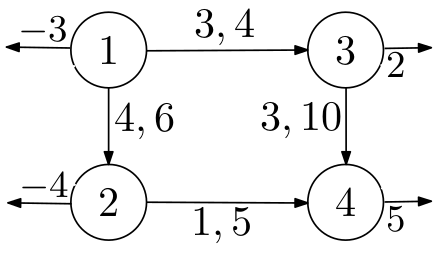
\includegraphics[width=0.5\textwidth]{img/rete_non_rilassata.png}
  \end{center}
  Si aggiungono i nodi fittizi $s$ e $t$ con sbilanciamento rispettivamente $b_s =b_1+b_2=-3-4 =-7$ e $b_t = b_3+b_4 = 2+5 =7$

  Si aggiungono gli archi fittizi con costo nullo e con capacità:
  \begin{itemize}
    \item $a_{s1} = -b_1 = 3$
    \item $a_{s2} = -b_2 = 4$
    \item $a_{3t} = b_3 = 2$
    \item $a_{4t} = b_4 = 5$
  \end{itemize}

  Si ottiene quindi la seguente rete rilassata:
  \begin{center}
    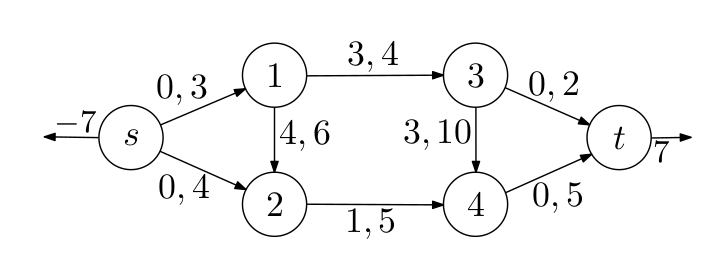
\includegraphics[width=0.5\textwidth]{img/rete_rilassata.png}
  \end{center}
}

Alle volte, inoltre, è utile che anche i nodi abbiano delle \textbf{capacità}, ossia che solo che solo una quantità di flusso compresa nell’intervallo chiuso $[l_i , u_i]$ possa passare per il nodo $i \in N$. Per fare ciò occorre \textit{sdoppiare} ciascun nodo $i$ in due nodi $i',i''$, in modo che:
\begin{itemize}
  \item Tutti gli archi entranti in $i$ entrino in $i'$ 
  \item tutti gli archi uscenti da $i$ escano da $i''$
  \item Si aggiunge un arco da $i'$ a $i''$ con capacità $[l_i,u_i]$
\end{itemize}
\begin{center}
  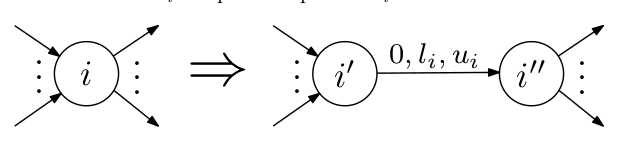
\includegraphics[width=0.5\textwidth]{img/giga_archetto_con_capacity.png}
\end{center}

\subsection{Problema di Flusso Massimo}

\dfn{Problema di Flusso Massimo}{
  Si definisce \textit{problema di flusso massimo} il problema di flusso in cui la funzione obbiettivo è il flusso da massimizzare e le cui capacità inferiori sono nulle
}
Ciò che cambia, quindi, dal problema di flusso di costo minimo è la funzione obbiettivo, che diventa, si vuole infatti \textit{massimizzare} il flusso, e non minimizzare il costo. 

Formalmente, data una rete $G = (N,A)$:
\begin{itemize}
  \item Si fissano due nodi $s$ e $t$ rispettivamente sorgente e pozzo
  \item  Si vuole trovare il massimo valore $v$ tale che se $b_s=-v, \, b_t=v$ e $b_i=0$ allora esiste un flusso ammissibile $x$ tale che $Ex=b$
\end{itemize}

Formalizzato in programmazione lineare, il problema di flusso massimo diventa:
\begin{equation}
  \begin{aligned}
  \max \quad & v \\
  \sum_{(j,s) \in BS(s)} x_{js} + v &= \sum_{(s,j) \in FS(s)} x_{sj}; \\
  \sum_{(j,i) \in BS(i)} x_{ji} - \sum_{(i,j) \in FS(i)} x_{ij} &= 0, \quad i \in N - \{s, t\}; \\
  \sum_{(j,t) \in BS(t)} x_{jt} &= \sum_{(t,j) \in FS(t)} x_{tj} + v; \\
  0 \leq x_{ij} &\leq u_{ij}, \quad (i,j) \in A.
  \end{aligned}
\end{equation}

\nt{
  Si noti che il problema di flusso massimo e' un caso particolare di problema di flusso di costo minimo, di fatti partendo da un problema di flusso massimo si puo' costruire un problema di flusso di costo minimo:
  \begin{itemize}
    \item Si nullificano i costi
    \item Si pone $l_{ij} = 0$ e $u_{ij} = \infty$
  \end{itemize}
}
  
\section{Problema del flusso massimo: algoritmi}

\subsection{Tagli}

\dfn{Taglio}{
  Si definisce \textbf{taglio} in una rete $G=(N,A)$ una coppia $(N',N'')$ di sottoinsiemi di $N$ tali che $N' \cup N'' = N$ e $N' \cap N'' = \emptyset$
}

Si noti, inoltre anche questa defnizione
\dfn{$(s,t)$-taglio}{
  Si definisce \textbf{$(s,t)$-taglio} in una rete $G=(N,A)$ un taglio ($N_s, N_t$) dove $s \in N_s$ e $t \in N_t$
}

Si prendi in considerazione inoltre i confini il confine fra gli $(s,t)-\text{tagli}$, dove:
\begin{itemize}
  \item $A^+(N_s, N_t) = \{(i,j) \in A \mid i \in N_s \land j \in N_t\}$ sono gli archi che vanno dalla partizione $s$ a $t$
  \item $ A^-(N_s,N_t)=\{(i,j)\in A\mid i\in N_t\land j\in N_s\} $ sono gli archi che vanno da $t$ a $s$
\end{itemize}



Adesso introduciamo un importante lemma sui tagli:
\mlenma{}{
  $\forall (s,t)-\text{taglio }(N_s,N_t)$ e $\forall$ flusso ammissibile $x$ con valore $v$, si ha che:
  \begin{itemize}
    \item $v = \sum_{(i,j)\in A^+(N_s,N_t)}x_{ij}- \sum_{(i,j)\in A^-(N_s,N_t)}x_{ij}$
    
    Si ha, quindi, che $v$ la somma del flusso uscente da $s$ meno il flusso entrante in $s$ 
    \item $v\leq \sum_{(i,j)\in A^+(N_s, N_t)} u_{ij}$
    
    Ovvero Il flusso massimo è sempre minore o uguale alla capacità totale del taglio
  \end{itemize}
}
\pf{Dimostrazione}{
  \begin{itemize}
    \item Dimostro la prima parte:
    Per definizione di $v$, si ha che:
    \[
      v = \sum_{(i,j)\in A}x_{ij} - \sum_{(i,j)\in A}x_{ji}
    \]
    Questo valore è uguale alla somma netta in uscita $\forall i\in N_s$ verso la partizione $N_t$, quindi:
    \[
      \sum_{(i,j)\in A}x_{ij} - \sum_{(i,j)\in A}x_{ji} = \sum_{k\in N_s}\left( \sum_{(k,j)\in A}x_kj-\sum_{(i,k)\in A}x_{ik} \right)
    \]
    E questa somma  è ovviamente uguale al flusso uscente dal confine $A^+(N_s, N_t)$ meno il flusso entrante dal confine $A^-(N_s, N_t)$, quindi:
    \[
      \sum_{k\in N_s}\left( \sum_{(k,j)\in A}x_kj-\sum_{(i,k)\in A}x_{ik} \right) = \sum_{(i,j)\in A^+(N_s,N_t)}x_{ij}- \sum_{(i,j)\in A^-(N_s,N_t)}x_{ij}
    \]
  
    Per riassumenre quindi:
    \begin{equation}
      v = \sum_{(i,j)\in A^+(N_s,N_t)}x_{ij}- \sum_{(i,j)\in A^-(N_s,N_t)}x_{ij}
    \end{equation}
    \item Dimostro la seconda parte:
    
    Ovvio perché è una semplice del punto 1
  \end{itemize}
}

% \end{document}
